
%%% Local Variables: 
%%% mode: latex
%%% TeX-master: t
%%% End: 

\chapter{凸包围体生成算法}
\label{cha:kcbp-construction}
从\ref{sec:convex-bv}可以看出包围体的紧致程度直接影响算法的效率,对于不规则形体, 常见的包围体往往不够紧致,凸包紧致但往往包含过多的面片数而增加算法的复杂性。

本文提出一种构造凸包围多面体的方法,该方法首先利用近似内凸包和~$k$-means~聚类算法生成构成凸包围多面体~$k$~个截面的法向。
然后根据输入点集沿各法向搜索切点构成截面, 最后由这些截面通过对偶映射的方式求交构成凸包围多面体。
该方法的主要优势是:
\begin{inparaenum}[1)]
\item 对给定点集可构造紧致的包围体;
\item 利用~GPU~加速,能够快速构造包围体;
\item 通过参数~$k$~调节凸包围多面体的简单性和紧致性,可适用于不同的应用场景。
\end{inparaenum}

由~$k$~个截面构成的凸包围多面体称为凸包围~$k$~面体($k$-Convex Bounding Polytope, 简称~$k$-CBP), 可通过~$k$~个半空间定义:
\begin{equation}
\label{equ:kcbp_definition}
\left\{
\begin{array}{l}
    k\mbox{-CBP} = \mathop  \bigcap \limits_{i = 1}^k \bm{H_i} \\
    \bm{H_i} = \left\{ {\left. {\bm{p} \in {\mathbb{R}^3}} \right| \bm{n_i} \cdot \bm{p} \le {w_i}} , w_i \in \mathbb{R} \right\},
\end{array}
\right.
\end{equation}

其中,$\bm{n_i}$~是半空间~$\bm{H_i}$~的法向,方向指向包围体外部,
$w_i$~是输入点集中沿~$\bm{n_i}$~方向投影的最大值。
如图\ref{fig:bunny}所示是~Bunny~模型的凸包围~34~面体(34-CBP)。

\begin{figure}[H] 
\centering
  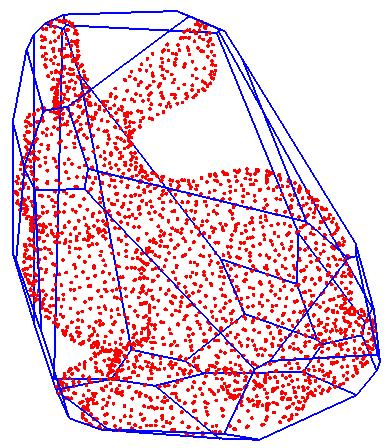
\includegraphics[width=1.3in]{bunny-34.png}
  \caption{~Bunny~模型的~34-CBP }
  \label{fig:bunny}
\end{figure}

本文提出的算法主要流程如图~\ref{lbl:kcbp-algorithm-flowchart}~
所示,首先利用近似内凸包和~$k$-means~聚类算法生成构成凸包围多面体~$k$~个截面的法向,然后根据输入点集在~GPU~中沿各法向搜索切点构成截面,
最后由这些截面通过对偶映射的方式求交构成凸包围多面体。搜索截面需要多次扫描输入点集,在~CPU~中计算较耗时,因此用~GPU~加速使得算法整体性能得以提升,其他步骤在~CPU~计算即可。

\begin{figure}[H]
    \centering
    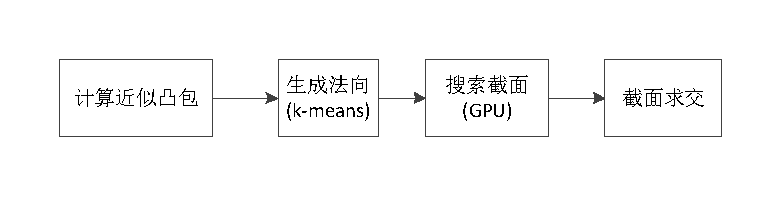
\includegraphics[height=0.7in]{kcbp-flowchart-x-aix.pdf}
    \caption{算法流程图}
    \label{lbl:kcbp-algorithm-flowchart}
\end{figure}

图\ref{lbl:bunny-26-cbp-ch-ach}~
从左至右分别显示了~Bunny~模型的~26-CBP、精确凸包和近似内凸包。近似凸包是精确凸包的一种近似,与精确凸包外观相似但其构造复杂度降低,不少研究者利用该性质解决计算机图形学中很多问题
\cite{hossain2013constructing}。本文就是利用近似内凸包与精确凸包的相似性,从众多近似凸包面片的法向中通过聚类算法生成凸包围多面体的~$k$~个法向。
%由图可知, 近似内凸包的三角面片大致反映了精确凸包三角面片的分布情况,近似内凸包相应位置面积较大的三角面片对应到精确凸包的三角面片面积也较大, 因此该三角面片所在平面需尽量保留.
\begin{figure}[H] % use [h] to fix the position
\centering
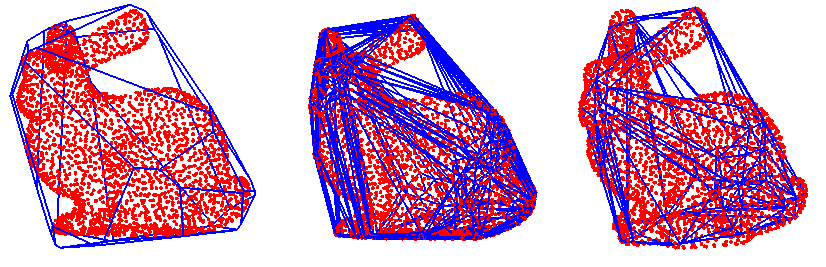
\includegraphics[width=5.0in]{26-bunny-ach-ch-kcbp.png}
\caption{~Bunny~模型的~26-CBP、凸包和近似内凸包}
\label{lbl:bunny-26-cbp-ch-ach}
\end{figure}
本章将按步骤详细介绍算法的实现。

\section{截面法向的生成}
\label{sec:gen-normals}

截面法向的选定与多面体的紧致程度密切相关。
$k$-DOP预先定义~$k/2$对法向,且$k$值局限于6、14、18或26等少数几个,导致其生成的多面体不能自适应模型,对于不规则形体不够紧致。相比本文$k$值取值更灵活,因此可以根据不同需求不同应用场景更加灵活地计算出凸包围体。
根据经验,为了使凸包围多面体尽可能逼近凸包,在多面体数量一定的情况下需尽量保留凸包中面积较大的面。 
本文算法先通过一种线性算法\cite{bentley1982approximation}构造近似内凸包,然后从近似内凸包里选取面积最大的~$a$~个面的法向,最后用聚类算法从剩下的面中生成~$k-a$~个法向。

\subsection{近似内凸包生成聚类样本法向集}
\label{subsec:ach-gen-normals}

下面以平面点集的近似内凸包为例说明初始法向集的生成。
\begin{figure}[H]
  \centering
  \subcaptionbox{Place points in bin\label{lbl:subfig-split-groups}}{
    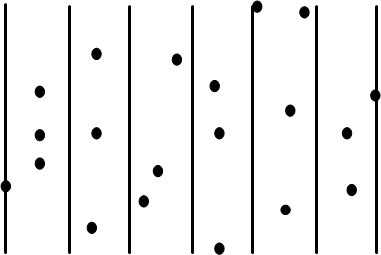
\includegraphics[width=1.7in]{approximate-convexhull-step1.png}} \hspace{0.5cm}
  \subcaptionbox{Find extremes in bins \label{lbl:subfig-find-extrems}}{%
    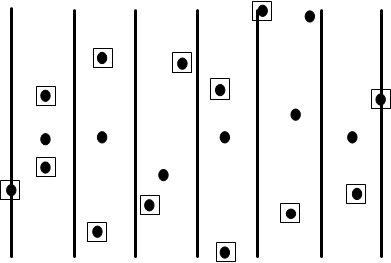
\includegraphics[width=1.7in]{approximate-convexhull-step2.png}} \hspace{0.5cm}
  \subcaptionbox{Choose extremes to build approximate hull\label{lbl:subfig-connect-extremes}}{%
    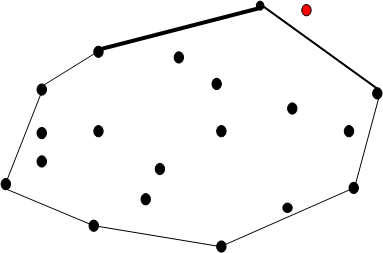
\includegraphics[width=1.7in]{approximate-convexhull-step3.png}} \hspace{0.5cm}
  \caption{二维近似内凸包的构造\cite{bentley1982approximation}}
\label{lbl:ach-2d}
\end{figure}

如图\ref{lbl:ach-2d}所示,整个算法分为3个步骤:
\begin{inparaenum}[(1)]
\item \textbf{分组。}
首先根据~$x$~轴将输入点均分~$\xi$~组,如图\ref{lbl:subfig-split-groups}所示,$\xi$值可以根据输入点集数量以及希望得到的近似凸包的近似程度进行选取,图示中分成了6组。
\item \textbf{选极值点。}
然后在每组中找出沿~$y$~轴的最大最小值,得到每组的极值点,如图\ref{lbl:subfig-find-extrems}所示,在边界上的点可直接当作极值点。
\item \textbf{连线。}
最后按条件连接每组的最值构成近似内凸包,如图\ref{lbl:subfig-connect-extremes}所示。//TODO,可更详细
\end{inparaenum}
此算法复杂度为~$O(n+\xi)$。  
得到近似凸包后,因较长的边(图中的粗边)对最后凸包围多边形影响较大, 因此可以保留较长的$a$条边(2D 为例), 其他$n-a$(n为近似内凸包边数)进行聚类得到$k-a$ 类, 最后得到边对应的垂直向外的方向作为法向。
在三维空间里, 可按照~$x,y$~轴最多划分成 $(\xi+2)\times (\xi+2)$个网格, 每个网格取~$z$~的最大最小值, 因此所有网格含最多有~$2(\xi+2)^2$~个极值点, 其凸包可以在$O(\xi^2\log \xi^2) = O(\xi^2\log \xi)$ 内找出, 因此整个算法时间复杂度为$O(n+\xi^2\log\xi)$, 
关于此算法更详细的细节可参考文献\onlinecite{bentley1982approximation}。 实验过程中, 为了更快地构造近似内凸包, $\xi$~值通常取得较小(例如取~$\xi=10$)。

假设点~$A,B,C$~为近似凸包的某个平面$P_i$上逆时针方向上的3个顶点,则该平面~$P_i$的法向$\bm{n_i}
= \overrightarrow{AB} \times
\overrightarrow{AC}$,这些法向就是参与聚类算法的所有样本法向集。


\subsection{聚类初始点的选择}
\label{subsec:initial-normals}

聚类算法是数据挖掘领域里的研究热点之一,$k$-means~是最流行和最简单的基于划分的聚类算法\cite{Jain2010}。其中,$k$-means
算法最初的步骤就是初始聚类中心的选择。本文算法将采取如下的策略生成:给定一个单位球,将其按照等面积划分成$k$份即$k$-means中的参数$k$,连接球心到每份中心点构成的方向作为法向,其效果如图\ref{lbl:kmeans-init-normals-26}所示($k=26$)。

\begin{figure}[H]
    \centering
    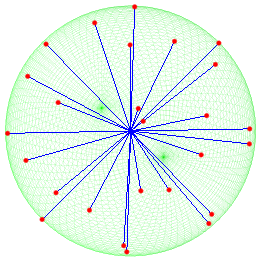
\includegraphics[height=1.7in]{kmeans-init-normals-26.png}
    \caption{初始聚类法向的生成}
    \label{lbl:kmeans-init-normals-26}
\end{figure}

初始点生成算法具体如算法~\ref{alg:get_init_normals_by_area}~所示\footnote{http://www.cmu.edu/biolphys/deserno/pdf/sphere\_equi.pdf}。
另外,亦可使用如文献\onlinecite{wong1997sampling}中的数学统计方法在球面上生成若干个点使其满足均匀分布。

\begin{algorithm}[H]
\algsetup{linenosize=\tiny}
\small
\caption{初始法向的生成}
\label{alg:get_init_normals_by_area}
\begin{algorithmic}[1]
\REQUIRE
初始法向数量:$k$
\ENSURE
~$k$~个法向:Normal
\STATE $i \gets 0$; $area \leftarrow 4\pi / k$
\STATE $m\_v \gets round(\pi/\sqrt{area})$
\STATE $d\_v \gets \pi/m\_v$
\STATE $d\_phi \gets area/d\_v$
\FOR {$m=0$ \TO $m\_v-1$}
    \STATE $v \gets \pi m/m\_v$
    \STATE $m\_phi \gets round(2\pi\sin{v}/d\_phi)$
    \FOR {$n=0$ \TO $m\_phi-1$}
        \STATE $\phi \gets 2\pi n/m\_phi$
        \STATE $Normal_i \gets vec3(\sin{v}\cos{\phi},\sin{v}\sin{\phi},\cos{v})$
        \STATE $i \gets i+1$
    \ENDFOR
\ENDFOR
\RETURN $Normal$
\end{algorithmic}
\end{algorithm}

 
\subsection{聚类确定法向}
\label{subsec:determ-normals}

聚类算法将相似程度高的变量聚集到一类,距离度量是$k$-means中的关键,采用不同的距离计算函数可能得到不同的聚类结果,依据数据的不同性质可选用不同的距离度量方法,常用的有欧式距离,曼哈顿距离和卡方距离等等。
本文采用余弦距离度量,将方向相近的点归聚到一类。$k$-means~本质上是一个迭代贪心算法,每一次迭代需要重新计算每一类的中心点,直到两次迭代后中心点相差在预定的容差范围内为止。
本文聚类更新中心点时将面片的面积作为权重即
\begin{equation}
\label{equ:kmeans-update-center}
\bm{c_i}=\frac{\sum_{i=1}^{i=n} \omega_i \cdot \bm{n_i} } {\sum_{i=1}^{i=n} \omega_i}
,
\end{equation}
其中$\bm{c_i}$
为第~$i$~类的中心点,$\omega_i$~为法向~$\bm{n_i}$~所在面片对应的面积,这样使得生成的法向尽量靠近原始近似凸包面积较大的面片的方向。完整的算法如算法~\ref{alg:kmeans-determine-normals}所示。

\begin{algorithm}
\algsetup{linenosize=\tiny}
\small
\caption{$k$-means确定法向}
\label{alg:kmeans-determine-normals}
\begin{algorithmic}[1]
\REQUIRE
初始中心点 $init$, 聚类数量 $k$, 聚类样本法向集 $points$
\ENSURE
~$k$~个聚类后的法向 $result$

\FORALL {$p \in points$}
    %\STATE $tmp \gets -\infty $
    \FORALL {$c \in init$}
        \STATE $\phi \gets c \cdot p$ \COMMENT{计算余弦距离, 并记录每个聚类变量属于哪一类}
        %\STATE $tmp \gets max(tmp, \phi)$ \COMMENT{记录每个聚类变量属于哪一类}
    \ENDFOR
    \FORALL {$c \in init$}
        \STATE $result \gets update(c)$ \COMMENT{按照公式\ref{equ:kmeans-update-center}更新中心点}
    \IF{$chk\_state(result, init, iter)$}
        \RETURN {$result$}
        \COMMENT{检测迭代条件是否满足,中心点容差范围内不在变化或迭代次数超过最大迭代次数}
    \ELSE
        \STATE $init \gets result $
        \STATE $iter \gets iter+1 $
    \ENDIF
    \ENDFOR
\ENDFOR
\end{algorithmic}
\end{algorithm}


通过聚类后得到的法向生成包围体比直接用初始法向生成的包围体更加紧致。如图~\ref{lbl:kemans-fixed-kcbp}~所示, 
其中图~\ref{lbl:fixed-kcbp-bunny}~为按照初始方向为~Bunny~模型生成的凸包围多面体($k=26$),
聚类后其法向及其生成的凸包围多面体如图~\ref{lbl:kmeans-kcbp-bunny}~所示, 后者的紧致程度比前者高~14.98\%.

\begin{figure}[H]
\setcounter{subfigure}{0}
  \centering
  \subcaptionbox{初始法向生成$k$-CBP\label{lbl:fixed-kcbp-bunny}}{%
    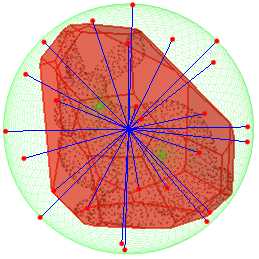
\includegraphics[width=1.8in]{kmeans-init-normals-26-for-bunny.png}}\hspace{3em}%
  \subcaptionbox{聚类法向生成$k$-CBP\label{lbl:kmeans-kcbp-bunny}}{%
    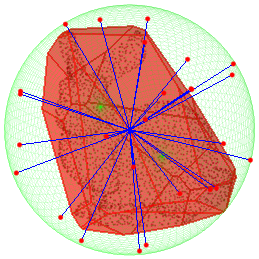
\includegraphics[width=1.8in]{kmeans-cluster-normals-26-for-bunny.png}}\hspace{3em}%
  \caption{初始法向和聚类确定法向生成$k$-CBP对比($k=26$)}
  \label{lbl:kemans-fixed-kcbp}
\end{figure}

\section{搜索截面}
\label{sec:search-planes}

在确定构成~$k$-CBP~的法向后,只需要搜索空间上的一个点即可确定
~$k$-CBP~的截面,搜索截面等效于寻找沿着法向上的最大投影值,即对每个法向~$\bm{n_i}$,从输入模型的所有点中寻找最大投影值的点作为切点进而确定~$\bm{n_i}$~对应的截面。
算法如算法~\ref{alg:search-plans-cpu}所示,该过程的算法复杂度为~$O(k\cdot
n)$, 其中~$k$~为法向数量, $n$~为模型所含点数。


\begin{algorithm}[H]
\algsetup{linenosize=\tiny}
\small
\caption{搜索截面串行算法}
\label{alg:search-plans-cpu}
\begin{algorithmic}[1]
\REQUIRE
截面法向 $normal$
模型点集 $points$
\ENSURE
多面体截面 $planes$

\FORALL {$\bm{n} \in normals$}
    \FORALL {$\bm{p} \in points$}
        \STATE $proj \gets  \bm{p} \cdot \bm{n}$ \COMMENT{计算投影值}
        \STATE $max\_proj \gets max(proj, max\_proj)$ \COMMENT{更新最大投影值}
    \ENDFOR
\ENDFOR
\FORALL {$\bm{n} \in normals$}
    \STATE $max\_point \gets \bm{n} \cdot max\_proj$ \COMMENT{切点}
    \STATE $planes\gets planes \cap plane(\bm{n}, max\_point)$ \COMMENT{构造平面}
\ENDFOR
\RETURN $planes$
\end{algorithmic}
\end{algorithm}

从算法~\ref{alg:search-plans-cpu}~可以看出该搜索过程中各法向的计算相互独立,因此可借助~GPU~并行加速。

\subsection{基于着色器的并行算法}
\label{subsec:determ-normals-by-shader}

OpenGL~提供了可编程管线,它的轻便性、跨平台性和被广泛硬件厂家所支持使得OpenGL
着色语言(GLSL,OpenGL Shading Language)被广泛应用,在基于~GPU~的通用计算(GPGPU,General
Purpose Graphic Process Unit)中也发挥着重要作用。下面将分别介绍本文提出的基于深度缓冲(Z Buffer)和乒乓技术的算法。

\subsubsection{基于深度缓冲的算法}
	
在~OpenGL~中,当渲染~3D~模型时,深度测试是在片段着色器工作后的一个重要测试操作,当两个片段在相同的位置时,深度测试的目的是决定哪个片段将要保留下来,默认情况下,最前面即有较小(或较大,可设置)的~$z$~坐标值的片段将通过测试被保留下来。
每个片段的深度信息保存在深度缓冲中,当新的片段通过测试后将更新缓冲中的值。
我们充分利用了~OpenGL~的这种机制,算法每走一遍渲染流程将找出一个方向的切点,在顶点着色器中,将所有点的~$x,y$~坐标值设为一样,并将该点在法向上的投影作为~$z$~值即深度值,所有点经过深度测试后将只有~$z$~值最大的点被保留下来,该点就是沿着这个法向的切点。

在实际实现过程中需要注意默认情况下~OpenGL~处理$x$和$y$坐标值的范围是$[-1,1]$,而深度值需要映射到$[0,1]$。我们利用一张$k \times 1$ 大小的纹理保存结果,将第$i$个法向的切点保存在纹理的$(i,0)$坐标处,这样做的好处是每绘制一遍不用清除深度缓冲,最后可以一次性读取这个$k \times 1$大小的纹理得到结果。
如附件~\ref{app-sec:shader-z-buffer}~的着色器代码所示,~OpenGL~中利用齐次坐标处理渲染流程,因此我们利用前三个分量保存法向的$x,y,z$坐标值,第4个分量$w$保存法向的索引,在片段着色器中,只需要简单地输出切点的在输入点数组的索引即可。
通过绘制$k$遍,我们从大小为$k \times 1$的纹理中读出点索引以此就能确定$k$切平面,每绘制一遍得到1个切平面,当$k$值较大时,这个过程仍然比较耗时,从实验结果也能看出,这种算法适用于$k$值相对较小的情况。
	
\subsubsection{基于乒乓技术的算法}

渲染到纹理是一个非常重要的图形可视化技术,它能够帮助快速地渲染很多漂亮的结果,同时也是GPGPU重要组成部分。在基于OpenGL的GPGPU中,通常要将参与计算的数据通过CPU传送至GPU的特定大小的纹理中,通过绘制一个跟保存数据同样大小的四边形来调用着色器中的算法\cite{gpgpuqiu},将结果输出到纹理中,绘制同样大小的四边形是为了避免纹理插值对输入数据的影响。
算法一般是在片段着色器(Fragment Shader)中完成,有些时候通过一遍的绘制得不到最终结果还希望把前一次运算结果传递给下一个运算用来作为后继运算的输入,此时可以利用乒乓技术来解决。

图~\ref{fig:shader-rrt-pingpong-flowchart}~为基于乒乓技术的算法的流程图,算法将所有法向保存在纹理$read$中并利用纹理$write$缓存中间结果,第$m$次渲染进行计算时,纹理$read$作为输入,将渲染即计算的结果缓存在纹理$write$中,在第$m+1$次渲染时将读取缓存在纹理$write$中的数据作为输入,而此时纹理$read$又作为输出,如此进行交替,每步交换只更换沿着每个法向的局部最大值。
如附件\ref{app-sec:shader-rtt-pingpong}~片段着色器代码所示,用一个像素值保存法向的xyz坐标值和沿着该法向投影得到最大值,另外用一个像素的第四个分量保存该最大值点在输入点数组中的索引。算法将输入点分成x份,每次只处理一份,在当前渲染过程中,找出在该批点中沿着所有法向投影值最大的点,当处理下批点集即下一次渲染时,将与上次局部最大投影值进行比较,若有新的投影最大值就更新,如此反复x次,当所有点都被处理完毕后得到沿着所有法向投影最大值的点即切点。最后再通过CPU一次性从帧缓冲中读取所有法向的切点。

\begin{figure}[H]
  \centering
  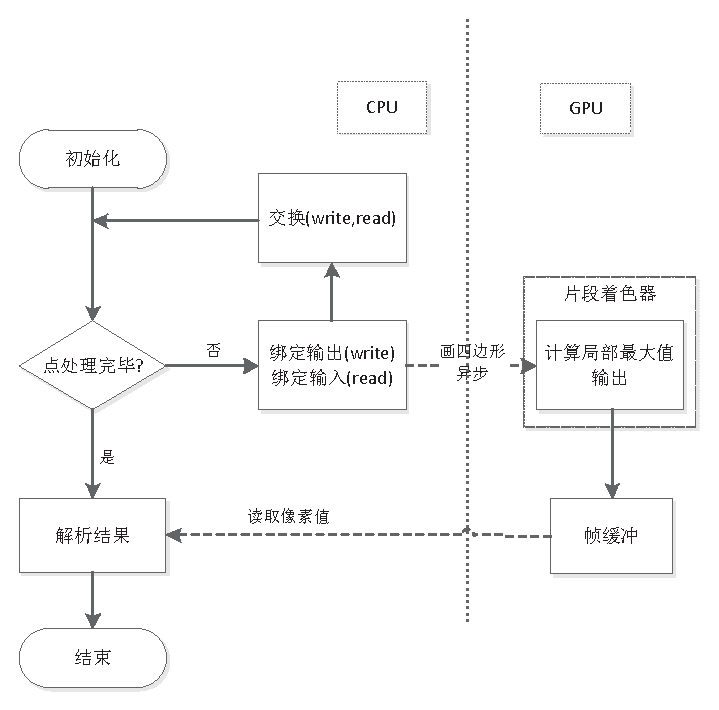
\includegraphics[width=4.0in]{shader-rtt-pingpong.eps}
  \caption{基于乒乓技术算法流程图}
  \label{fig:shader-rrt-pingpong-flowchart}
\end{figure}

与Z Buffer算法相比,基于乒乓技术的算法在进行一次绘制操作能够得到沿着k个法向的局部(所有处理过的点集)最大值。为了充分利用GPU的并行计算能力,将每次处理点的数量设置为GPU硬件所支持的OpenGL中统一块(uniform
block)所能容纳数据的大小,即需要反复绘制次数$x=n/b$,其中n为点集大小,b为统一块能容纳点的数量,值与显卡具体型号有关。 

\subsection{基于~CUDA~的并行算法}
\label{subsec:determ-normals-by-cuda}

~CUDA~是显卡公司~NVIDIA~推出的通用的并行计算架构平台,能够利用GPU解决并行计算问题,并提供了多种语言的编程接口。
\begin{figure}[H] % use [h] to fix the position
\centering
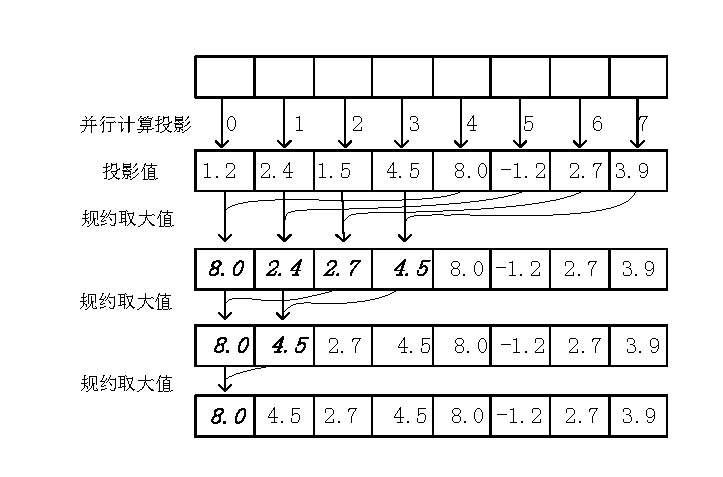
\includegraphics[width=4.0in]{gpureduction.pdf}
\caption{并行规约求最大投影值}
\label{lbl:reduction-getmax}
\end{figure}
如图\ref{lbl:reduction-getmax}~
所示,最大投影值的计算可采用如下规约方式:将输入点交给数量为~$t$~的线程计算点积得到投影值,
线程~$i$~和~$i +
t/2$~比较选取较大者,经~$\log_2t$~次比较可得最大值。更多更详细规约优化技术可参考文献~\onlinecite{Harris2007Optimizing}。

\section{截面求交算法}
\label{sec:intersect-planes}

确定$k$-CBP~各个截面后,直接求的所有平面交点并排除掉在平面外部的交点即可得到$k$-CBP~的顶点。即问题转化为:给定$k$个平面及其法向,平面及法向相当于一个半空间~$\bm{H}$,即已知集合${\bm{H_1},
\bm{H_2}, \cdots, \bm{H_k}}$,求$\bm{H_1} \cap \bm{H_2} \cap \cdots
\cap \bm{H_k}$。该问题是一个线性规划(Linear
Programming)问题,文献\onlinecite{dengcg}~详细介绍了在二维线性规划下的相关算法,本文将分别采用一种直观的枚举算法和利用对偶映射的方法求得$k$-CBP的交点。

\subsection{枚举法}
\label{subsec:intersection-enum-geometry}

空间中的平面位置情况如图~\ref{fig:three-planes-intersection}~所示,
若3个平面互相平行则没有交点,如图~\ref{lbl:intersection-center-0}~;
或者相交于1条交线,如图~\ref{lbl:intersection-center-1}~;
当有两个平面互相平行,另一个平面与其相交时有2条交线,如图~\ref{lbl:intersection-center-2}~;
亦或交于3条交线,如图~\ref{lbl:intersection-center-3}~;
最后一种情况是三个平面相交于1点的情况,如图~\ref{lbl:intersection-center-4}~所示。一个凸多面体的每一个顶点都可看作是至少3个平面的交点。现在只需要枚举出所有3个平面相交于1点的所有情况即可得到$k$-CBP~的顶点,值得注意的是,并非所有交点都是多面体的顶点,交点在某个半空间的正方向上即在半空间相交区域的外部须排除。

\begin{figure}[H]
\setcounter{subfigure}{0}
  \centering
  \subcaptionbox{没有交点\label{lbl:intersection-center-0}}{%
    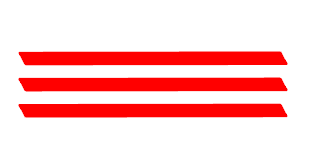
\includegraphics[width=1.5in]{intersection-center-0.png}}\hspace{1em}%
  \subcaptionbox{交于~1~条线\label{lbl:intersection-center-1}}{%
    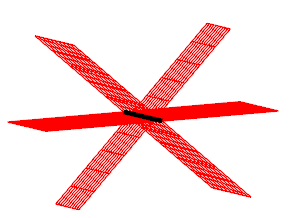
\includegraphics[width=1.5in]{intersection-center-1.png}}\hspace{1em}%
  \subcaptionbox{交于~2~条线\label{lbl:intersection-center-2}}{%
    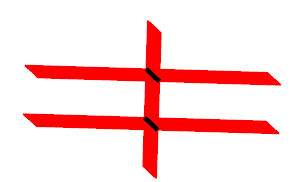
\includegraphics[width=1.5in]{intersection-center-2.png}}%
  \\
  \subcaptionbox{交于~3~条线\label{lbl:intersection-center-3}}{%
    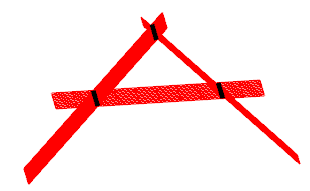
\includegraphics[width=2.0in]{intersection-center-3.png}}%
  \subcaptionbox{交于~1~个点\label{lbl:intersection-center-4}}{%
    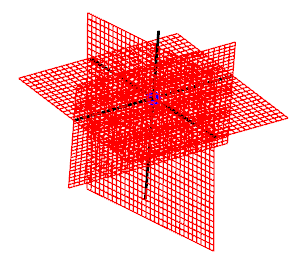
\includegraphics[width=1.7in]{intersection-center-4.png}}%
  \caption{空间中~3~个平面的相交情况}
  \label{fig:three-planes-intersection}
\end{figure}

假设满足如图~\ref{lbl:intersection-center-4}~的三个平面的法向分别是$\bm{n_1}, \bm{n_2}, \bm{n_3}$,
点$\bm{p_1}, \bm{p_2}, \bm{p_3}$,则三个平面的交点须满足如下方程: 

\begin{equation}
  \label{equa:three-planes-intersection}
  \left\{
    \begin{array}{l}
      \bm{n_1} \cdot \bm{x} = \bm{n_1} \cdot \bm{p_1}\\
      \bm{n_2} \cdot \bm{x} = \bm{n_2} \cdot \bm{p_2}\\
      \bm{n_3} \cdot \bm{x} = \bm{n_3} \cdot \bm{p_3}
    \end{array}
    \right.
\end{equation}

令$(\bm{n_1} \cdot \bm{p_1}, \bm{n_2} \cdot \bm{p_2}, \bm{n_3} \cdot \bm{p_3})
= (y_1, y_2, y_3) = \bm{y}$,则公式~\ref{equa:three-planes-intersection}~相当于解线性方程组
$\bm{A} \bm{x}=\bm{y}$ 即 $(\bm{n_1},\bm{n_2}, \bm{n_3})^T \cdot \bm{x} = \bm{y}$, 令
$\bm{n_i} = (a_{i1}, a_{i2}, a_{i3}), i=\{1,2,3\}$,则有:
\begin{equation*}
  \label{equa:matrix:crammer}
  \left(
    \begin{array}{ccc}
      a_{11} & a_{12} & a_{13} \\
      a_{21} & a_{22} & a_{23} \\
      a_{31} & a_{32} & a_{33} \\
    \end{array}
  \right)
  \cdot 
  \bm{x} 
 % \left(
 %   \begin{array}{c}
 %     x_{1} \\
 %     x_{2} \\
 %     x_{3} \\
 %   \end{array}
 % \right)
  =
  \left(
    \begin{array}{c}
      y_{1} \\
      y_{2} \\
      y_{3} \\
    \end{array}
  \right)
\end{equation*}
根据克莱姆法则(Crammer's Rule),上述方程有唯一解,则
$|\bm{A}| \not= 0$,且解~$x_i = \frac{|\bm{A_i}|}{|\bm{A}|}, i =
\{1,2,3\}$,其中$\bm{A_i}|$是矩阵A中将第i列替换成$\bm{y}^T$之后的行列式,在计算$\bm{A_i}$和$|\bm{A}|$时为了避免一些重复计算,将其展开有:

\begin{equation*}
 \left\{
\begin{array}{llll}
%\begin{aligned}
    |\bm{A}|   &=
    a_{11}  \left|
                  \begin{array}{cc}
                    a_{22} & a_{23} \\
                    a_{32} & a_{33} \\
                  \end{array}
              \right|
    &- a_{12} \left|
                  \begin{array}{cc}
                    a_{21} & a_{23} \\
                    a_{31} & a_{33} \\
                  \end{array}
              \right|
    &+ a_{13}
              \left|
                  \begin{array}{cc}
                    a_{21} & a_{22} \\
                    a_{31} & a_{32} \\
                  \end{array}
              \right|
\vspace{0.5em}\\ \vspace{0.5em}
    |\bm{A}_1| &= 
    y_1     \left|
                  \begin{array}{cc}
                    a_{22} & a_{23} \\
                    a_{32} & a_{33} \\
                  \end{array}
              \right|
    &- a_{12} \left|
                  \begin{array}{cc}
                    y_2 & a_{23} \\
                    y_3 & a_{33} \\
                  \end{array}
              \right|
    &+ a_{13}
              \left|
                  \begin{array}{cc}
                    y_2 & a_{22} \\
                    y_3 & a_{32} \\
                  \end{array}
              \right|
\\ \vspace{0.5em}
    |\bm{A}_2| &= 
    a_{11}  \left|
                  \begin{array}{cc}
                    y_{2} & a_{23} \\
                   y_{3} & a_{33} \\
                  \end{array}
              \right|
    &- y_{1}  \left|
                  \begin{array}{cc}
                    a_{21} & a_{23} \\
                    a_{31} & a_{33} \\
                  \end{array}
              \right|
    &+ a_{13}
              \left|
                  \begin{array}{cc}
                    a_{21} & y_{2} \\
                    a_{31} & y_{3} \\
                  \end{array}
              \right|
\\ \vspace{0.5em}
    |\bm{A}_3| &= 
    a_{11}  \left|
                  \begin{array}{cc}
                    a_{22} & y_{2} \\
                    a_{32} & y_{3} \\
                  \end{array}
              \right|
    &- a_{12} \left|
                  \begin{array}{cc}
                    a_{21} & y_{2} \\
                    a_{31} & y_{3} \\
                  \end{array}
              \right|
    &+ y_{1}
              \left|
                  \begin{array}{cc}
                    a_{21} & a_{22} \\
                    a_{31} & a_{32} \\
                  \end{array}
              \right|
\end{array}
%\end{aligned}
\right.
\end{equation*}

令
$b_1 = \left|
\begin{array}{cc}
  a_{22} & a_{23} \\
  a_{32} & a_{33} 
\end{array} 
\right|
  = a_{22}a_{33} - a_{32}a_{23}
,
b_2 = \left|
\begin{array}{cc}
  a_{21} & a_{23} \\
  a_{31} & a_{33} 
\end{array} 
\right|
  = a_{21}a_{33} - a_{31}a_{23}
,
b_3 = \left|
\begin{array}{cc}
  a_{21} & a_{22} \\
  a_{31} & a_{32} \\
\end{array}
\right|
= a_{21}a_{32}-a_{31}a_{22}
,
b_4 = \left|
  \begin{array}{cc}
    y_2 & a_{23} \\
    y_3 & a_{33} \\
  \end{array}
\right|
  = y_2a_{33}-y_3a_{23}
,
b_5 = \left|
  \begin{array}{cc}
      y_2 & a_{22} \\
      y_3 & a_{32} \\
      \end{array}
    \right|
  = y_2a_{32}-y_3a_{22}
,
b_6 = \left|
    \begin{array}{cc}
      a_{21} & y_{2} \\
      a_{31} & y_{3} \\
    \end{array}
  \right|
  =a_{21}y_{3}-a_{31}y_{2}
$, 则有:
\begin{equation}
  \label{equa:solution:three-planes}
  \left\{
    \begin{array}{lll}
      x_1 =& \frac{|\bm{A_1}|}{|\bm{A}|} =&\frac{y_1b_1-a_{12}b_4+a_{13}b_5}{a_{11}b_1-a_{12}b_2+a_{13}b_3} 
      \vspace{0.5em}\\ \vspace{0.5em}
      x_2 =& \frac{|\bm{A_2}|}{|\bm{A}|} =&\frac{a_{11}b_4-y_{1}b_2+a_{13}b_6}{a_{11}b_1-a_{12}b_2+a_{13}b_3} 
      \\ \vspace{0.5em}
      x_3 =& \frac{|\bm{A_3}|}{|\bm{A}|} =&\frac{-a_{11}b_5-a_{12}b_6+y_{1}b_3}{a_{11}b_1-a_{12}b_2+a_{13}b_3}
    \end{array}
  \right.
\end{equation}其中,$|\bm{A}| \not= 0$。


\begin{algorithm}[H]
\algsetup{linenosize=\tiny}
\small
\caption{枚举算法}
\label{alg:enum_algortihm}
\begin{algorithmic}[1]
\REQUIRE
平面:$planes$
\ENSURE
凸包围多面体:$k$-CBP

\FORALL {$p_1 \in planes$}
  \STATE $Intersection \gets \emptyset $
  \FORALL {$p_2 \in planes$}
        \FORALL {$p_3 \in planes$}
            %\IF{$ (p_1 = p_2 || p_1 = p_3 || p_2 = p_3) = \FALSE $}
            \IF{$ p_1 \nparallel p_2 \nparallel p_3$}
                \IF{$|A| \not= 0$}
                    \STATE $P = (x_1, x_2, x_3)$
                    \COMMENT{按照公式~\ref{equa:solution:three-planes}~计算得到交点坐标值} 
                    \IF{$validate(P)$}
                      \STATE $Intersection \gets Intersection \cup P$
                      \COMMENT{验证交点P是否都在半空间负方向上}
                    \ENDIF
                \ENDIF
            \ENDIF
        \ENDFOR
   \ENDFOR
   \IF {$Intersection.size \geq 3$}
   \STATE {$k\textrm{-CBP} \gets k\textrm{-CBP} \cup poly(p_1, Intersection)$}
   \COMMENT{满足条件,加入到结果集}
   \ENDIF
\ENDFOR
\RETURN {$k$-CBP}
\end{algorithmic}
\end{algorithm}

完整的算法如算法~\ref{alg:enum_algortihm}~所示,枚举遍历所有平面的组合,搜索出三个平面交于1点的情况,排除在半空间外部的交点即可得到~$k$-CBP~的顶点,算法复杂度为~$O(n^3)$。

\subsection{对偶映射算法}
\label{subsec:intersection-dual-mappint}

确定截面后对其进行对偶映射求凸包, 该凸包面映射的点即为原始截面的交点即凸包围多面体的顶点, 方法如下:每个平面经对偶映射成一个三维点, 例如平面由法向~$\bm{n}(a,b,c)$~及平面上一点~$\bm{p}(x_0,y_0,z_0)$~确定, 转化为平面方程~$ax + by + cz = ax_0 + by_0 + cz_0=d$, $d \neq 0$.
对偶映射后的点为~$\bm{p'}(a/d, b/d, c/d)$, 然后通过对这~$k$~个映射点求凸包, 最后将凸包的每个平面转换即可得到原始平面的交点, 此算法的时间复杂度为$O(k\log k$), 在利用对偶映射求交点时要注意原始模型需包含原点.

\section{实验结果}
\label{sec:exper-kcbp}
